\documentclass[11pt,a4paper,fleqn]{article}
\usepackage[utf8]{inputenc}
\usepackage{bsymb}
%usepackage[space]{ctex}
\usepackage{natbib}
\usepackage{graphicx}
\usepackage{algorithmic_pf}
\usepackage{indentfirst}
\usepackage[export]{adjustbox}
\usepackage{etoolbox}
\expandafter\patchcmd\csname Gin@ii\endcsname
  {\setkeys {Gin}{#1}}
  {%
    \setkeys {Gin}
      {max width=\textwidth,max height=.5\textwidth,keepaspectratio,#1}%
  }
  {}{}
\title{Homework 4,5}

\author{10175101126,10175101226,10175101117}
\date{April 2019}
\setkeys{Gin}{max width=\linewidth}
\begin{document}
\maketitle

\section{ homework 2.4 }
\subsection{Rewrite PRE and POST }
\noindent
$ PRE: n > 0,f\in 0 \upto n-1 \rightarrow N $\\
POST:g \in 0 \upto n-1 \rightarrow N , \forall i \cdot i \in 0 \upto n-1 \Rightarrow g(i)=f(n-i-1) \\
%\setlength{\hangindent}{2em}



\subsection{Prove the invariants}
\noindent
Prove the invariant: g \in 0 \upto n-1 \rightarrow N \\
PRE \vdash [g:=f] g \in 0 \upto n-1 \rightarrow N \quad INI \\
n>0,f \in 0 \upto n-1 \vdash f \in 0 \upto n-1 \quad HYP \\
PRE,i<j,g \in 0 \upto n-1 \rightarrow N \vdash [g :=(\{i, j\} \domsub g) \cup\{i \mapsto g(j), j \mapsto g(i)\}]g \in 0 \upto n-1 \rightarrow N \quad INV \quad HYP\\
\noindent
\\
Prove \; the \; invariant: i \in 0 \upto n-1 \\
Pre \vdash [i:=0]i \in 0 \upto n-1 \quad INI \\
Pre \vdash 0 \in 0 \upto n-1 \\
n > 0 \vdash 0 \in 0 \upto n-1 \quad \\
PRE,i<j,i+j=n-1,i\in 0 \upto n-1 ,j\in 0 \upto n-1 \vdash [i:=i+1]i\in 0 \upto n-1 \; INV \\
Before\;it, \; prove \; the \; auxiliary \; lemma \; \\
PRE,i<j,i+j=n-1,i\in 0 \upto n-1  \vdash i \neq n-1 \\
PRE,i=n-1,i<j,i \in 0 \upto n-1 ,j \in 0 \upto n-1 \vdash i+j\neq n-1 \;CT2 \\
PRE,i=n-1,i<j,j \in 0 \upto n-1 \vdash j \notin 0 \upto n-1 \;AH \\
PRE,i=n-1,i<j,i \in 0 \upto n-1 ,j \in 0 \upto n-1,j \notin 0 \upto n-1 \vdash i+j \neq n-1 \;CT1 \\
The\;auxiliary\;lemma\;has\;been\; proved \\
PRE,i<j,i+j=n-1,i\in 0 \upto n-1 ,i\neq n-1 ,j\in 0 \upto n-1 \vdash [i:=i+1]i\in 0 \upto n-1 \; AH \\
PRE,i<j,i+j=n-1,i\in 0 \upto n-1 ,i\neq n-1 ,j\in 0 \upto n-1 \vdash i+1 \in 0 \upto n-1 \\


\noindent
Prove \; the \; invariant:  j \in 0 \upto n-1\\
PRE \vdash [j:=n-1]j \in 0 \upto n-1 \;INI \\
PRE \vdash n-1 \in 0 \upto n-1 \\
Before\;it, \; prove \; the \; auxiliary \; lemma \; \\
n>0 \vdash n-1 \geq 0 \\
Obvious \\
PRE,n-1 \geq 0 \vdash [j:=n-1]j \in 0 \upto n-1 \;AH \\
PRE,n-1 \geq 0 \vdash n-1 \in 0 \upto n-1 \\
Then\;prove \\
PRE,i<j,i \in 0 \upto n-1 ,j \in 0 \upto n-1,i+j=n-1\vdash [j:=j-1]j\in 0 \upto n-1 \;INV \\
Before\;it, \; prove \; the \; auxiliary \; lemma \; \\
PRE,i<j,i \in 0 \upto n-1 ,j \in 0 \upto n-1,i+j=n-1\vdash j\neq 0 \\
PRE,i<j,i \in 0 \upto n-1 ,j \in 0 \upto n-1,j=0 \vdash i+j\neq n-1\; CT2 \\
PRE,i<j,i \in 0 \upto n-1 ,j \in 0 \upto n-1,j=0 \vdash i \notin 0 \upto n-1\\
PRE,i<j,i \in 0 \upto n-1 ,i \notin 0 \upto n-1,j \in 0 \upto n-1,j=0 \vdash i+j\neq n-1\; AH \; CT1 \\
Then\;prove \\
PRE,i<j,i \in 0 \upto n-1 ,j \in 0 \upto n-1,i+j=n-1,j\neq 0 \vdash [j:=j-1]j\in 0 \upto n-1 \;AH \\
PRE,i<j,i \in 0 \upto n-1 ,j \in 0 \upto n-1,i+j=n-1,j\neq 0 \vdash j-1 \in 0 \upto n-1 \\


\noindent
Prove the invariant: i+j=n-1 \\
PRE \vdash [i:=0,j:=n-1]i+j=n-1 \;INI \\
PRE \vdash 0+n-1=n-1 \\
PRE,i<j,i+j=n-1 \vdash [i:=i+1,j:=j-1]i+j=n-1 \;INV \\
PRE,i<j,i+j=n-1 \vdash i+1+j-1=n-1 \\
PRE,i<j,i+j=n-1 \vdash i+j=n-1 \; HYP \\

\noindent
Prove the invariant: i\leq j+1 \\
PRE \vdash [i:=0,j:=n-1]i \leq j+1 \;INI \\
n>0 \vdash 0 \leq n \;HYP \\
PRE,i<j,i \leq j+1,i \in 0 \upto n-1 ,j \in 0 \upto n-1 \vdash [i:=i+1,j:=j-1]i\leq j+1 \;INV \\
PRE,i<j,i \leq j+1,i \in 0 \upto n-1 ,j \in 0 \upto n-1 \vdash i+1 \leq j \;HYP\\

\noindent
Prove the invariant: \forall k \cdot k \in 0 \upto i-1 \Rightarrow g(k)=f(n-k-1) \\
PRE \vdash [i:=0]\forall k \cdot k \in 0 \upto i-1 \Rightarrow g(k)=f(n-k-1) \;INI\\
PRE \vdash \forall k \cdot k \in 0 \upto -1 \Rightarrow g(k)=f(n-k-1) \;CT1 \\
set\; \boldsymbol{h}=(\{i, j\} \domsub g) \cup\{i \mapsto g(j), j \mapsto g(i)\} \\
Then\;prove \\
PRE,i<j,i+j=n-1,g :=h \vdash [i:=i+1,g:=h] \forall k \cdot k \in 0 \upto i-1 \Rightarrow g(k)=f(n-k-1) \;INV \\
\noindent
[g:=h]\forall k \cdot k \in 0 \upto i \Rightarrow g(k)=f(n-k-1) \\
\forall k \cdot k \in 0 \upto i-1 \Rightarrow h(k)=f(n-k-1),\forall \boldsymbol{k} \cdot \boldsymbol{k} \in \boldsymbol{i} \upto j \Rightarrow h(\boldsymbol{k})=\boldsymbol{f}(\boldsymbol{k}) \vdash \forall k \cdot k \in 0 \upto i \Rightarrow h(k)=f(n-k-1) \;SPLIT \\
First \;case\; k=i \\
h(i)=g(j) \\
\forall k \cdot k \in i \upto j \Rightarrow g(k) = f(k),i+j=n-1 \vdash \ g(j) = f(n-i-1) \\
g(j)=f(j),j+i=n-1\vdash g(j)=f(n-i-1) \;UH \\
g(j)=f(n-i-1)\vdash g(j)=f(n-i-1) \; HYP \\
Second \; case \; k \in 0 \upto i-1 \\
\forall k \cdot k \in 0 \upto i-1 \Rightarrow h(k)=f(n-k-1) \vdash h(k)=f(n-k-1) \;HYP \\

\noindent
Prove the invariant: \forall k \cdot k \in i \upto j \Rightarrow g(k)=f(k) \\
PRE \vdash [g:=f]\forall k \cdot k \in i \upto j \Rightarrow g(k)=f(k) \;INI \\
PRE \vdash \forall k \cdot k \in i \upto j \Rightarrow f(k)=f(k) \\
PRE,i<j,\forall k \cdot k \in i \upto j \Rightarrow g(k)=f(k) \vdash [i:=i+1,j:=j-1]\forall k \cdot k \in i \upto j \Rightarrow g(k)=f(k) \\
PRE,i<j,\forall k \cdot k \in i \upto j \Rightarrow g(k)=f(k) \vdash \forall k \cdot k \in i+1 \upto j-1 \Rightarrow g(k)=f(k) \\
PRE,i<j,\forall k \cdot k \in i \upto j \vdash k \in i+1 \upto j-1 \\
PRE,i<j,\forall k \cdot k \in i \upto j \Rightarrow g(k)=f(k), k \in i+1 \upto j-1 \vdash \forall k \cdot k \in i+1 \upto j-1 \Rightarrow g(k)=f(k) \;AH\\

\noindent
Prove the invariant:\forall k \cdot k \in j+1 \upto n-1 \Rightarrow g(k) = f(n-k-1) \\
set\; \boldsymbol{h}=(\{i, j\} \domsub g) \cup\{i \mapsto g(j), j \mapsto g(i)\} \\
PRE \vdash [j:=n-1]\forall k \cdot k \in j+1 \upto n-1 \Rightarrow g(k) = f(n-k-1) \;INI \\
PRE \vdash \forall k \cdot k \in n \upto n-1 \Rightarrow g(k) = f(n-k-1) \;CT1 \\
PRE,i<j,\forall k \cdot k \in j+1 \upto n-1 \Rightarrow g(k) = f(n-k-1) \vdash [j:=j-1,g:=h]\forall k \cdot k \in j+1 \upto n-1 \Rightarrow h(k) = f(n-k-1) \;INV \\
PRE,i<j,\forall k \cdot k \in j+1 \upto n-1 \Rightarrow g(k) = f(n-k-1) \vdash \forall k \cdot k \in j \upto n-1 \Rightarrow h(k) = f(n-k-1)  \\
First\;case\;k=j\\
h(j)=g(i) \\
\forall k \cdot k \in i \upto j \Rightarrow g(k) = f(k),i+j=n-1 \vdash \ g(j) = f(n-i-1) \\
g(i)=f(i),j+i=n-1\vdash g(i)=f(n-j-1) \;UH \\
g(i)=f(n-j-1)\vdash g(i)=f(n-j-1) \; HYP \\
Second\;case\;k\in j+1\upto n-1 \\
PRE,i<j,\forall k \cdot k \in j+1 \upto n-1 \Rightarrow g(k) = f(n-k-1) \vdash \forall k \cdot k \in j+1 \upto n-1 \Rightarrow g(k) = f(n-k-1) \;HYP\\


\subsection{ Prove POST}
\noindent
$\ldots,g\in 0\upto n-1\rightarrow\mathbb{N}\vdash g\in 0\upto n-1\rightarrow\mathbb{N}\quad\text{HYP\quad and \quad SPLIT}$\\
\\
$ \ldots,i\leq j+1,i\geq j,i+j=n-1,$\\
$ \forall k\cdot k\in 0\upto i-1 \Rightarrow g(k)=f(n-1-k),$\\
$ \forall k\cdot k\in i\upto j \Rightarrow g(k)=f(k),$\\
$ \forall k\cdot k\in j+1\upto n-1 \Rightarrow g(k)=f(n-1-k)$\\
$\vdash \forall k\cdot k\in 0\upto n-1 \Rightarrow g(k)=f(n-1-k)$\\
\\
$ \ldots,(i=j) \lor (i=j+1),i+j=n-1,$\\
$ \forall k\cdot k\in 0\upto i-1 \Rightarrow g(k)=f(n-1-k),$\\
$ \forall k\cdot k\in i\upto j \Rightarrow g(k)=f(k),$\\
$ \forall k\cdot k\in j+1\upto n-1 \Rightarrow g(k)=f(n-1-k)$\\
$\vdash \forall k\cdot k\in 0\upto n-1 \Rightarrow g(k)=f(n-1-k)$\\
\\
$ \ldots,i=j,i+j=n-1,$\\
$ \forall k\cdot k\in 0\upto i-1 \Rightarrow g(k)=f(n-1-k),$\\
$ \forall k\cdot k\in i\upto j \Rightarrow g(k)=f(k),$\\
$ \forall k\cdot k\in j+1\upto n-1 \Rightarrow g(k)=f(n-1-k)$\\
$\vdash \forall k\cdot k\in 0\upto n-1 \Rightarrow g(k)=f(n-1-k)\quad\text{OR\_H}$\\
\\
$ \ldots,j=n-1-j,$\\
$ \forall k\cdot k\in 0\upto j-1 \Rightarrow g(k)=f(n-1-k),$\\
$ \forall k\cdot k\in j\upto j \Rightarrow g(k)=f(k),$\\
$ \forall k\cdot k\in j+1\upto n-1 \Rightarrow g(k)=f(n-1-k)$\\
$\vdash \forall k\cdot k\in 0\upto n-1 \Rightarrow g(k)=f(n-1-k)\quad\text{EQL}$\\
Obvious,since $j=n-1-j$ when $k=j$,we have $g(j)=f(j)=f(n-1-j)$\\
\\
$ \ldots,i=j+1,i+j=n-1,$\\
$ \forall k\cdot k\in 0\upto i-1 \Rightarrow g(k)=f(n-1-k),$\\
$ \forall k\cdot k\in i\upto j \Rightarrow g(k)=f(k),$\\
$ \forall k\cdot k\in j+1\upto n-1 \Rightarrow g(k)=f(n-1-k)$\\
$\vdash \forall k\cdot k\in 0\upto n-1 \Rightarrow g(k)=f(n-1-k)\quad\text{OR\_H}$\\
\\
$ \ldots,j=n-1-j-1,$\\
$ \forall k\cdot k\in 0\upto j+1 \Rightarrow g(k)=f(n-1-k),$\\
$ \forall k\cdot k\in j+1\upto j \Rightarrow g(k)=f(k),$\\
$ \forall k\cdot k\in j+1\upto n-1 \Rightarrow g(k)=f(n-1-k)$\\
$\vdash \forall k\cdot k\in 0\upto n-1 \Rightarrow g(k)=f(n-1-k)\quad\text{EQL}$\\
Obvious,$(j+1\upto j)=\mathbb{\phi}$\\


\subsection{Propose a variant and prove it}
\noindent
since j-i decreased all the time,we choose j-i as the variant.\\
\\
$\text{NAT:}$\\
$\ldots,i<j\vdash j-i\in \mathbb{N}$\quad since $j-i>0$\\
$\text{VAR:}$\\
$ \ldots,i<j\vdash [i:=i+1;j:=j-1]j-i<j-i$\\
$ \ldots,i<j\vdash [i:=i+1][j:=j-1]j-i<j-i$\\
$ \ldots,i<j\vdash [i:=i+1]j-1-i<j-i$\\
$ \ldots,i<j\vdash j-1-i-1<j-i$\\
$ \ldots,i<j\vdash -2<0$


\subsection{Translate this program to C and execute it}
\noindent
Program is listed here:
\begin{figure}[h!]
\centering
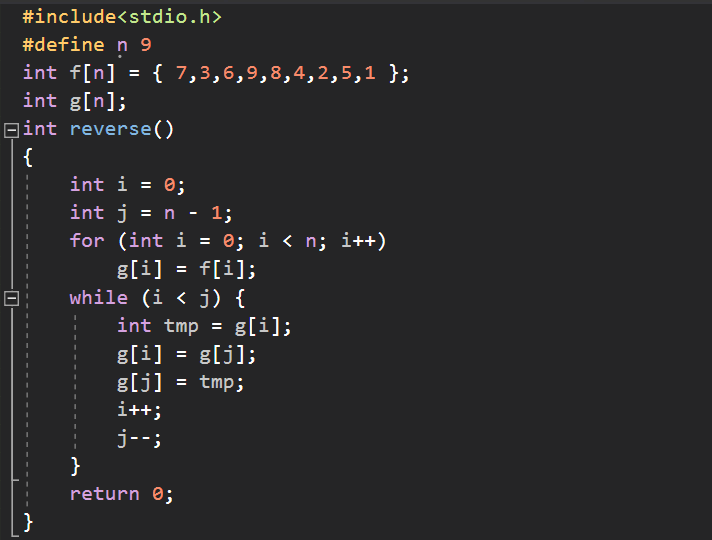
\includegraphics{1.png}
\caption{ write in c}
\label{fig}
\end{figure}
\begin{figure}[h!]
\centering
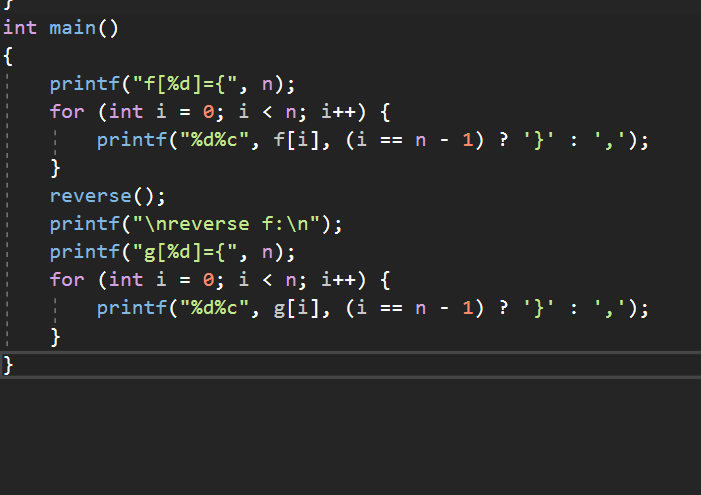
\includegraphics{2.png}
\caption{ write in c}
\label{fig}
\end{figure}
\begin{figure}[h!]
\centering
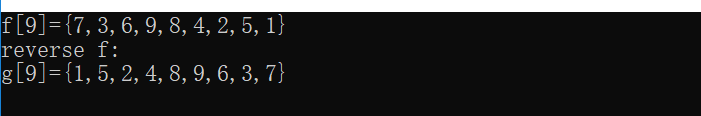
\includegraphics{3.png}
\caption{ run }
\label{fig}
\end{figure}

\section{homework 2.5}

\subsection{Exercise 1: terminate this proof}
\noindent
case1:\\
$m \in (k + 1)+1 \upto j$\\
$\forall m \cdot m \in k+1 \upto j \Rightarrow g(m) > x  $\\
$\forall m \cdot m \in 0 \upto k \Rightarrow g(m) \leq x $\\
$g(j+1) \leq x $\\
$\vdash$\\
$h(m)>x $\\

\noindent
where h is $ (\{k+1, j+1\} \domsub g) \cup\{k+1 \mapsto g(j+1), j+1 \mapsto g(k+1)\}$\\
\noindent so we have:\\
$h(m) = g(m)$ since $m>k+1 $ and $m<j+1$\\ 
\noindent Applying rule \text{U}\_\text{H}:\\
$g(m)>x $\\
$ \forall m \cdot m \in 0 \upto k \Rightarrow g(m) \leq x $\\
$g(j+1) \leq x $\\
$m \in (k + 1)+1 \upto j$\\
$\vdash$\\
$g(m)>x \quad \text{HYP}$\\

\noindent
case2($m = j+1 $):\\
$\forall m \cdot m \in k+1 \upto j \Rightarrow g(m) > x  $\\
$\forall m \cdot m \in 0 \upto k \Rightarrow g(m) \leq x $\\
$g(j+1) \leq x $\\
$ \vdash$ \\
$h(j+1)>x \quad \text{EQL} $\\
\noindent
where h is $ (\{k+1, j+1\} \domsub g) \cup\{k+1 \mapsto g(j+1), j+1 \mapsto g(k+1)\}$\\
\noindent so we have $h(j+1)=g(k+1)$\\
\noindent Applying $\text{U}\text{\_}\text{H}$\\
$\g(k+1) > x  $\\
$\forall m \cdot m \in 0 \upto k \Rightarrow g(m) \leq x $\\
$g(j+1) \leq x $\\
$ \vdash$ \\
$g(k+1)>x \quad \text{HYP} $\\

\subsection{Exercise 2: terminate this proof}
\noindent
The last assumption leads to a proof by cases:\\
$m \in 0 \upto k$ and $m = k+1$\\

\noindent
Case1($m \in 0 \upto k $):\\
$\forall m \cdot m \in k+1 \upto j \Rightarrow g(m) > x  $\\
$\forall m \cdot m \in 0 \upto k \Rightarrow g(m) \leq x $\\
$g(j+1) \leq x $\\
$m \in 0 \upto k $\\
$ \vdash$ \\
$h(m) \leq x $\\
\noindent
where h is $ (\{k+1, j+1\} \domsub g) \cup\{k+1 \mapsto g(j+1), j+1 \mapsto g(k+1)\}$\\
So we have $g(m)=h(m) $ since $ m<k+1$ and obvious $ k<=j $.\\
Then applying rule \text{U}\_\text{H}:\\
$\forall m \cdot m \in k+1 \upto j \Rightarrow g(m) > x  $\\
$ g(m) \leq x $\\
$g(j+1) \leq x $\\
$m \in 0 \upto k $\\
$ \vdash$ \\
$h(m) \leq x \quad \text{HYP}$\\

\noindent
Case2($m=k+1$):\\
$\forall m \cdot m \in k+1 \upto j \Rightarrow g(m) > x  $\\
$\forall m \cdot m \in 0 \upto k \Rightarrow g(m) \leq x $\\
$g(j+1) \leq x $\\
$m = k +1 $\\
$ \vdash$\\
$h(k+1) \leq x\quad \text{EQL} $\\

\noindent
where h is $ (\{k+1, j+1\} \domsub g) \cup\{k+1 \mapsto g(j+1), j+1 \mapsto g(k+1)\}$\\
So we have $ h(k+1) = g(j+1)$, therefore:\\
$\forall m \cdot m \in k+1 \upto j \Rightarrow g(m) > x  $\\
$\forall m \cdot m \in 0 \upto k \Rightarrow g(m) \leq x $\\
$g(j+1) \leq x $\\
$ \vdash$\\
$g(j+1) \leq x \quad \text{HYP}$\\


\subsection{Exercise 3}

\subsubsection{Rewrite PRE and POST conditions}
\noindent
PRE: \\
$$ n>0$$ $$ f \in 0 \upto n-1 \rightarrow \mathbb{N}$$ $$ x \ge 0$$

\noindent
POST:\\
$$k \in -1 \upto n-1 $$ $$ g \in 0 \upto n-1 \rightarrow \mathbb{N}$$
$$ ran(f) =ran(g) $$ $$ \forall m \cdot m \in 0 \upto k \Rightarrow g(m) \leq x $$ $$\forall m \cdot m \in k+1 \upto n-1 \Rightarrow g(m) > x  $$

\subsubsection{Prove all invariants}
\noindent
1. $ j \in -1 \upto n-1$\\
\text{INI}\\
$PRE,\ldots \vdash [k:=-1,j:=-1,g:=f](j\in -1 \upto n-1) $\\
$PRE,\ldots \vdash -1 \in -1 \in n-1 $\\
obvious since we have $n>0$.\\
\text{INV}\\
when $g(j+1)>x$,\\
$PRE,\ldots,j \not= n-1,g(j+1)>x  \vdash [j:=j+1](j\in -1 \upto n-1) $\\
$PRE,\ldots,j \not= n-1,g(j+1)>x,j\in -1 \upto n-1  \vdash j+1\in -1 \upto n-1 $\\
$PRE,\ldots,j+1\in -1 \upto n-1 \vdash j+1\in -1 \upto n-1 \quad \text{HYP}$\\

\noindent
when $g(j+1) \leq x$,\\
$PRE,\ldots,j \not= n-1,g(j+1) \le x,j\in -1 \upto n-1 \vdash [g :=(\{k+1, j+1\} \domsub g) \cup\{k+1 \mapsto g(j+1), j+1 \mapsto g(k+1)\},j:=j+1,k:=k+1](j\in -1 \upto n-1) $\\
$PRE,\ldots,j \not= n-1,j\in -1 \upto n-1  \vdash j+1\in -1 \upto n-1 $\\
$PRE,\ldots,j+1\in -1 \upto n-1 \vdash j+1\in -1 \upto n-1 \quad \text{HYP}$\\

\noindent
2. $k \in -1 \upto j$\\
\text{INI}\\
$PRE,\ldots \vdash [k:=-1,j:=-1,g:=f](k \in -1 \upto j) $\\
$PRE,\ldots \vdash -1 \in -1 \upto j$\\
obvious $j \ge -1$\\
\text{INV}\\
when $g(j+1)>x$,\\
$PRE,\ldots,j \not= n-1,g(j+1)>x,k \in -1 \upto j  \vdash [j:=j+1](k \in -1 \upto j) $\\
$PRE,\ldots,j \not= n-1,g(j+1)>x,k \in -1 \upto j  \vdash k \in -1 \upto j \quad \text{HYP}$\\

\noindent
when $g(j+1) \le x$\\
$PRE,\ldots,j \not= n-1,g(j+1) \le x,k \in -1 \upto j \vdash [g :=(\{k+1, j+1\} \domsub g) \cup\{k+1 \mapsto g(j+1), j+1 \mapsto g(k+1)\},j:=j+1,k:=k+1](k \in -1 \upto j) $\\
$PRE,\ldots,j \in -1 \upto n-1 , j\not= n-1, k \in -1 \upto j \vdash k+1 \in -1 \upto j+1 $\\
obvious since $k \le j $ and $j \ge -1$.\\

\noindent
3. $g \in 0 \upto n-1 \rightarrow \mathbb{N}$\\
\text{INI}\\
$PRE,\ldots \vdash [k:=-1,j:=-1,g:=f](g \in 0 \upto n-1 \rightarrow \mathbb{N})$\\
$PRE,\ldots \vdash f \in 0 \upto n-1 \rightarrow \mathbb{N}$ \quad \text{HYP}\\
obvious in PRE.

\noindent
\text{INV}\\
when $g(j+1)>x$\\
$PRE,\ldots,j \not= n-1,g(j+1)>x,k \in -1 \upto j  \vdash [j:=j+1](g \in 0 \upto n-1 \rightarrow \mathbb{N}) $\\
$PRE,\ldots,g \in 0 \upto n-1 \rightarrow \mathbb{N},j \not= n-1,g(j+1)>x,k \in -1 \upto j  \vdash g \in 0 \upto n-1 \rightarrow \mathbb{N} \quad \text{HYP}$\\

\noindent
when $g(j+1) \le x$\\
$PRE,\ldots,j \not= n-1,g(j+1) \le x,k \in -1 \upto j  \vdash [g :=(\{k+1, j+1\} \domsub g) \cup\{k+1 \mapsto g(j+1), j+1 \mapsto g(k+1)\},j:=j+1,k:=k+1](g \in 0 \upto n-1 \rightarrow \mathbb{N}) $\\
$PRE,\ldots,g \in 0 \upto n-1 \rightarrow \mathbb{N},j \not= n-1,g(j+1)>x,k \in -1 \upto j  \vdash g \in 0 \upto n-1 \rightarrow \mathbb{N} \quad \text{HYP}$\\
%待斟酌

\noindent
4. $ranf(g) = ran(f)$\\
\text{INI}\\
$PRE,\ldots \vdash [k:=-1,j:=-1,g:=f](ranf(g) = ran(f)) $\\
$PRE,\ldots \vdash ranf(f) = ran(f) $\\
obvious since one should equal to itself.

\noindent
\text{INV}\\
when $g(j+1)>x$\\
$PRE,\ldots,j \not= n-1,g(j+1)>x,k \in -1 \upto j  \vdash [j:=j+1](ranf(g) = ran(f)) $\\
$PRE,\ldots,j \not= n-1,g(j+1)>x,ranf(g) = ran(f),k \in -1 \upto j  \vdash ranf(g) = ran(f) \quad \text{HYP}$\\

\noindent
when $g(j+1) \le x$\\
$PRE,\ldots,j \not= n-1,ran(f)=ran(g),g(j+1) \le x  \vdash [g :=(\{k+1, j+1\} \domsub g) \cup\{k+1 \mapsto g(j+1), j+1 \mapsto g(k+1)\},j:=j+1,k:=k+1](ran(f)=ran(g)) $\\
$PRE,\ldots,j \not= n-1,g(j+1)>x,ranf(g) = ran(f),k \in -1 \upto j  \vdash ranf(g) = ran(f) \quad \text{HYP}$\\
obvious since the range of f and g doesn't change. \\

\noindent
5. $\forall m \cdot m \in 0 \upto k \Rightarrow g(m) \le x$\\
\text{INI}\\
$PRE,\ldots \vdash [k:=-1,j:=-1,g:=f](\forall m \cdot m \in 0 \upto k \Rightarrow g(m) \le x)$\\
$PRE,\ldots \vdash \forall m \cdot m \in 0 \upto k \Rightarrow g(m) \le x$\\
% $PRE,\ldots,m \in 0 \upto k \vdash    f(m) \le x \quad \text{U}\_
% \text{G}$\\
$PRE,\ldots,\forall m \cdot m \in k+1 \upto j \Rightarrow g(m)>x,m \in 0 \upto k \vdash    f(m) \le x $\\
$PRE,\ldots,g(m) \le x,m \in 0 \upto k \vdash    g(m) \le x \quad \text{HYP}$\\

\noindent
\text{INV}\\
when $g(j+1)>x$\\
$PRE,\ldots,\forall m \cdot m \in 0 \upto k \Rightarrow g(m) \le x,j \not= n-1,\forall m \cdot m \in k+1 \upto j \Rightarrow g(m)>x,g(j+1)>x  \vdash [j:=j+1](\forall m \cdot m \in 0 \upto k \Rightarrow g(m) \le x) $\\
$PRE,\ldots,\forall m \cdot m \in 0 \upto k \Rightarrow g(m) \le x,\forall m \cdot m \in k+1 \upto j \Rightarrow g(m)>x,g(j+1)>x  \vdash \forall m \cdot m \in 0 \upto k+1 \Rightarrow g(m) \le x  $\\
$PRE,\ldots,\forall m \cdot m \in 0 \upto k \Rightarrow g(m) \le x,\forall m \cdot m \in k+1 \upto j \Rightarrow g(m)>x,m \in 0 \upto k  \vdash  g(m) \le x  \quad \text{U}\_\text{G}$\\
$PRE,\ldots,\forall m \cdot m \in 0 \upto k \Rightarrow g(m) \le x,m \in 0 \upto k  \vdash  g(m) \le x $\\
$PRE,\ldots,g(m) \le x  \vdash  g(m) \le x  \quad \text{HYP}$\\

\noindent
when $g(j+1) \le x$\\
$PRE,\ldots,\forall m \cdot m \in 0 \upto k \Rightarrow g(m) \le x,g(j+1) \le x,\forall m \cdot m \in k+1 \upto j \Rightarrow g(m)>x  \vdash [g :=(\{k+1, j+1\} \domsub g) \cup\{k+1 \mapsto g(j+1), j+1 \mapsto g(k+1)\},j:=j+1,k:=k+1](\forall m \cdot m \in 0 \upto k \Rightarrow g(m) \le x) $\\
$PRE,\ldots,\forall m \cdot m \in 0 \upto k \Rightarrow g(m) \le x,g(j+1) \le x,\forall m \cdot m \in k+1 \upto j \Rightarrow g(m)>x  \vdash \forall m \cdot m \in 0 \upto k+1 \Rightarrow h(m) \le x $\\
where h is $ (\{k+1, j+1\} \domsub g) \cup\{k+1 \mapsto g(j+1), j+1 \mapsto g(k+1)\}$\\
Applying rule U\_G:\\
$PRE,\ldots,\forall m \cdot m \in 0 \upto k \Rightarrow g(m) \le x,\forall m \cdot m \in k+1 \upto j \Rightarrow g(m)>x,m \in 0 \upto k+1  \vdash  h(m) \le x $\\
Please see the following proof of this at exercise 2.\\

\noindent
6. $\forall m \cdot m \in k+1 \upto j \Rightarrow g(m)>x$\\
\text{INI}\\
$PRE,\ldots \vdash [k:=-1,j:=-1,g:=f](\forall m \cdot m \in k+1 \upto j \Rightarrow g(m)>x$\\
$PRE,\ldots,\forall m \cdot m \in 0 \upto k \Rightarrow g(m) \le x, \vdash \forall m \cdot m \in k+1 \upto j \Rightarrow g(m)>x$\\
$PRE,\ldots,\forall m \cdot m \in 0 \upto k \Rightarrow g(m) \le x,m \cdot m \in k+1, \vdash  g(m)>x \quad \text{U}\_\text{G}$\\
$PRE,\ldots, g(m)>x \vdash  g(m)>x \quad \text{HYP}$\\

\noindent
\text{INV}\\
when $g(j+1)>x$\\
$PRE,\ldots,\forall m \cdot m \in 0 \upto k \Rightarrow g(m) \le x,j \not= n-1,\forall m \cdot m \in k+1 \upto j \Rightarrow g(m)>x,g(j+1)>x  \vdash [j:=j+1](\forall m \cdot m \in k+1 \upto j \Rightarrow g(m) > x) $\\
$PRE,\ldots,\forall m \cdot m \in 0 \upto k \Rightarrow g(m) \le x,\forall m \cdot m \in k+1 \upto j \Rightarrow g(m)>x \vdash \forall m \cdot m \in k+1 \upto j+1 \Rightarrow g(m) > x $\\
$PRE,\ldots,\forall m \cdot m \in 0 \upto k \Rightarrow g(m) \le x,\forall m \cdot m \in k+1 \upto j \Rightarrow g(m)>x, m \in k+1 \upto j+1 \vdash  g(m) > x $\\
therefore we split it into 2 situation,\\
when $m \in k+1 \upto j$\\
$PRE,\ldots,\forall m \cdot m \in 0 \upto k \Rightarrow g(m) \le x,\forall m \cdot m \in k+1 \upto j \Rightarrow g(m)>x, m \in k+1 \upto j \vdash  g(m) > x $\\
$PRE,\ldots,g(m) > x \vdash  g(m) > x  \quad \text{HYP}$\\
when $m = j+1$\\
$PRE,\ldots,\forall m \cdot m \in 0 \upto k \Rightarrow g(m) \le x,\forall m \cdot m \in k+1 \upto j \Rightarrow g(m)>x, m =j+1,g(j+1)>x \vdash  g(j+1) > x \quad \text{HYP}$\\

\noindent
when $g(j+1) \le x$\\
$PRE,\ldots,\forall m \cdot m \in 0 \upto k \Rightarrow g(m) \le x,j \not= n-1,\forall m \cdot m \in k+1 \upto j \Rightarrow g(m)>x,g(j+1) \le x  \vdash [g :=(\{k+1, j+1\} \domsub g) \cup\{k+1 \mapsto g(j+1), j+1 \mapsto g(k+1)\},j:=j+1,k:=k+1](\forall m \cdot m \in k+1 \upto j \Rightarrow g(m) > x) $\\
$PRE,\ldots,\forall m \cdot m \in 0 \upto k \Rightarrow g(m) \le x,j \not= n-1,\forall m \cdot m \in k+1 \upto j \Rightarrow g(m)>x,g(j+1) \le x  \vdash \forall m \cdot m \in (k+1)+1 \upto j+1 \Rightarrow h(m) > x $\\
where h is $ (\{k+1, j+1\} \domsub g) \cup\{k+1 \mapsto g(j+1), j+1 \mapsto g(k+1)\}$\\
Applying rule U\_G:\\
$PRE,\ldots,\forall m \cdot m \in 0 \upto k \Rightarrow g(m) \le x,j \not= n-1,\forall m \cdot m \in k+1 \upto j \Rightarrow g(m)>x,g(j+1) \le x, m \in (k+1)+1 \upto j+1  \vdash  h(m) > x $\\
The last assumption leads to a proof by cases:\\
$m \in (k+1)+1 \upto j$ and $m = j+1 $\\
Please see the following proof of this at exercise 1.\\


\subsubsection{Prove POST}
\noindent
$ \text{PRE},$
$j=n-1,$
$j\in -1\upto n-1,$
$k\in -1\upto j,$\\
$g\in 0\upto n-1\rightarrowtail\mathbb{N},$
$ran(g)=ran(f),$\\
$ \forall m \cdot m \in 0 \upto k \Rightarrow g(m) \leq x ,$\\
$ \forall m \cdot m \in k+1 \upto j \Rightarrow g(m)>x$\\
$\vdash$\\
$k\in -1\upto n-1,$
$g\in 0\upto n-1\rightarrowtail\mathbb{N},$
$ran(g)=ran(f),$\\
$ \forall m \cdot m \in 0 \upto k \Rightarrow g(m) \leq x ,$\\
$ \forall m \cdot m \in k+1 \upto n-1 \Rightarrow g(m)>x$\\
\\
$\text{PRE},$
$n-1\in -1\upto n-1,$
$k\in -1\upto n-1,$\\
$g\in 0\upto n-1\rightarrowtail\mathbb{N},$
$ran(g)=ran(f),$\\
$ \forall m \cdot m \in 0 \upto k \Rightarrow g(m) \leq x ,$\\
$ \forall m \cdot m \in k+1 \upto n-1 \Rightarrow g(m)>x$\\
$\vdash$\\
$k\in -1\upto n-1,$
$g\in 0\upto n-1\rightarrowtail\mathbb{N},$
$ran(g)=ran(f),$\\
$ \forall m \cdot m \in 0 \upto k \Rightarrow g(m) \leq x ,$\\
$ \forall m \cdot m \in k+1 \upto n-1 \Rightarrow g(m)>x\quad \text{HYP\quad and\quad EQL}$\\



\subsubsection{Propose a variant and prove it}
\noindent
since j increases all the time, we choose n-1-j as the variant.\\ 
\\
$\text{NAT:}$\\
$ \ldots,j\in -1\upto n-1\vdash n-1-j\in \mathbb{N}$\quad since $j\leq n-1$\\
$\text{VAR:}$\\
$ \ldots,g(j+1)>x\vdash[j:=j+1]n-1-j<n-1-j$\\
$ \ldots,g(j+1)>x\vdash n-1-(j+1)<n-1-j$\\
$ \ldots,g(j+1)>x\vdash -1<0$\\
Obvious since $-1<0$\\
$ \ldots,g(j+1)\leq x\vdash[j:=j+1;g:=h;k:=k+1]n-1-j<n-1-j$\\
$ \ldots,g(j+1)\leq x\vdash[j:=j+1][g:=h][k:=k+1]n-1-j<n-1-j$\\
$ \ldots,g(j+1)\leq x\vdash[j:=j+1][g:=h]n-1-j<n-1-j$\\
$ \ldots,g(j+1)\leq x\vdash[j:=j+1]n-1-j<n-1-j$\\
$ \ldots,g(j+1)\leq x\vdash n-1-j-1<n-1-j$\\
$ \ldots,g(j+1)\leq x\vdash -1<0$\\
Obvious since $-1<0$\\

\subsubsection{Translate the program to C and run it}
Program is listed here:\\

\begin{figure}[h!]
\centering
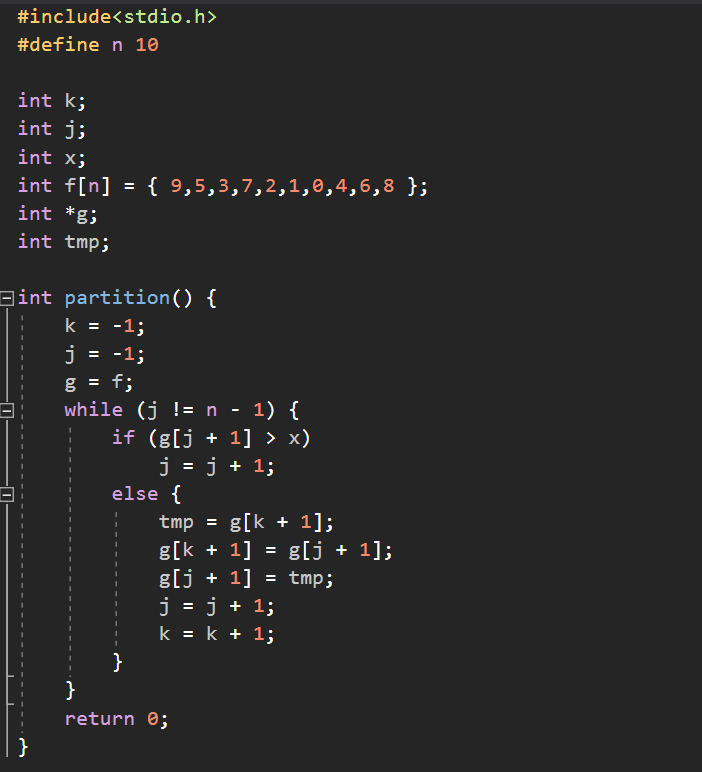
\includegraphics{4.png}
\caption{ write in c}
\label{fig}
\end{figure}

\begin{figure}[h!]
\centering
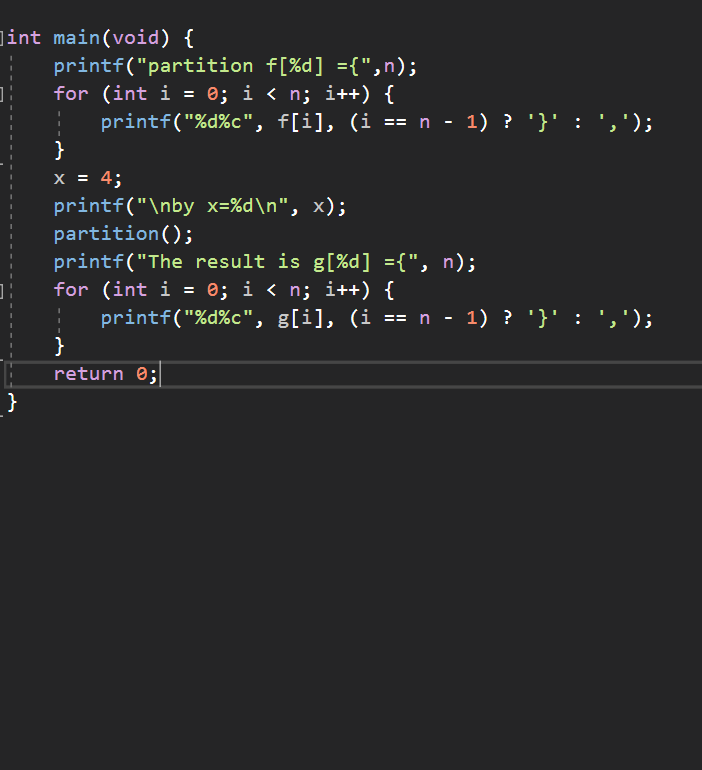
\includegraphics{5.png}
\caption{ write in c}
\label{fig}
\end{figure}

\begin{figure}[h!]
\centering
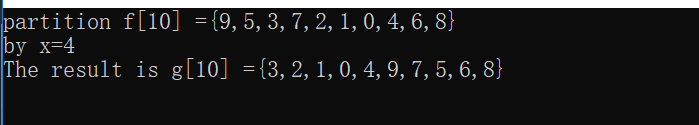
\includegraphics{6.png}
\caption{ run }
\label{fig}
\end{figure}



%\bibliographystyle{plain}
%\bibliography{references}
\end{document}
